\section{Results}

\subsubsection{Funding and Response Tone}
When separating out the questions on funding, who responded and response tone we can see several interesting trends. While the question asked several different ways that people could be paid for their contributions, it can be simplified to a binary attribute of paid / unpaid. In most cases, there were a mix of funding but in this analysis all that mattered was if there was any financial incentives. Additionally the responses to “How did the response read” formed a binary attribute as well with all participants selecting either Peer or Teacher.

Though there isn't much data to go by, in funded organizations more people reported the response tone to their initial contribution read as being answered as peers rather than as teachers. Further exploration shows that unlike unfunded projects, in paid organizations it was rarely the project founder who responded but rather a senior project member. This might explain the presence of a more peer-to-peer response tone verse a pedagogical response tone.

\subsubsection{True Motivations for Open Source Contribution}
{\bold 42. What do you want to get in return for your contribution?} My reason for asking about contributor motivation is to figure out if people really want anything in return for volunteering their time. Time is money, and it would be naive to think that everyone is truly altruistic. Out of 24 responses, a {\italic staggering} 50% want more experience in open source communities. This should be taken with a grain of salt because respondents are class peers. However, 25% are looking for career advancement or “nothing at all”, while a few receive satisfaction, skills, societal benefit, and web development experience from contributing. It is apparent that career advancement is a major reason for open source collaboration. Strangely enough, an equal amount of people want nothing at all, and only 2 respondents wanted academic recognition. Our sample size is small and academically biased, so it will be interesting extrapolate from a larger and more diverse sample size.


\subsubpararaph { Design and Previous Experiences }

In my experiences working on Hypothes.is for this class, a few questions had come to mind while I jumped into my first open source project. The first was trying to understand how difficult it would be for me to find a project that would suit my skills and what I'm looking for, since the only contribution I could really put forth was my design work. So some key quetsions that had arisen primarily involved how important design was to the project and what to expect from them. This tangentially led me to wonder how much experience others in the class had with open collaboration projects, since I felt that many had an easy time jumping into one or knowing what they wanted to do. I then felt like it was appropriate to ask the class these two pressing questions; "How important do you find design is to your project" and "what was your involvement with open source projects before this class". 

I was pleasantly surprised at the results I got. Many agreed that design was important to their project, with "I Agree" holding 61\% of the answers. I was more expecting a higher number of "I Somewhat Agree" which holds 35\% of the current answers. While I'm glad to know that many projects find design to be an important aspect of it, in hindsight I wonder if I should have rephrased the question to more analyze the role of the design team on the project. I felt like it was a given to understand that design is important, but it's another thing to actually see that the project actively prioritizes design by establishing an open collaborateive design team. 

The results for whether or not people had previous experience in open source projects did not surprise me, as many individuals seemed like they are generally active in this space. If anything I was slightly surprised by the number of "No" answers.




\mysubsubsection{The Difference between Experienced and Newcomers in Open Source}
To start my analysis, I divided the total number of responses into two categories based on how they answered the question : ``Prior to this project, did you have any experience in the past with open source projects?"
As a newcomer to open source communities myself, I wanted to analyze to {\bf see if there were any discernable differences or interesting trends between newcomers and ``veterans" of open source communities.} 
I started with the responses for how long did the individual lurk before making an attempt at reaching out to the community. We can see that in contrast to the ``No" group, the ``Yes" group has 2/11 or 18\% of people who didn't even lurk for a single day. On the  ``No" side, we can see that not  a single individual spent 0 days lurking and all of them had to spend at least 1-3 days lurking prior to joining.  This could indicate a stronger willingness to immediately dive in to a new Open Source community by the people who have had prior experience with them and a heightened shyness exhibited by the group with no experience with them before. The distribution for the YES  group is very disjoint when compared to the No group. For 71\%(5/7) of the Yes Group, it took them either more than a month or immediately to enter the OS community. This could indicate either {\it an extreme willingness or elongated hesitation that is not seen in the No Group} since there are no individuals that took 0 days and not as much of a frequency(20\% vs 43\%) of individuals that took more than 29+ days.  Statistically, {\it the distribution of the ``Yes" group is much more bimodal} with the peaks being at 0 days and 29+ days compared to the No group. 
 	Another interesting division between the two groups was their responses for the question ``what do  I plan on getting out of this contribution" For the Yes Group, the majority of them wanted not only experience in OS software but some sort of other reward like academic publication, career advancement, etc. However, this is decidedly false for the No Group where the majority wanted only experience in OS software or even nothing at all. This could be from the fact that because the Yes Group has contributed to Open Source communities before, they would need an extra incentive to join a new community while the No Group is simply excited to be part of this endeavor that they have never been on before. I think with further data, we could see if the requirement or desire for external incentives would increase linearly with the number of OS communities one would participate in.

Lastly, I thought it would be interesting to test if the two different groups would have differences in the roles that they play within their respective open source communities. I found that the number of roles a particular user from the Yes Group is significantly more than the number of roles a user from the No Group would take. This is to be expected as it is the No Group's first time. Other than that difference, the No Group had less developers and less documenters than the Yes Group but the same number of UX/Designers, Testers, and Analysts as the Yes Group. 


\subsubparagraph{From lurking to first contact}
Most of the participants answered that they {\bold have been lurking} prior to contacting the project, although the days of lurking are widely spread among the projects. {\italic 21%} answered that the question is not applicable for them and their project. 
About half of the people used mail to get into contact with the community (either through a private mail or to the mailing list). Social media was only used by one participant \foonote{Fogel pointed out that social networks might have an impact on OS, but the impact is still not well understood.}. This suggests that mail is still the main form of communication, at least for initial communication.

\subsubsection{Personal Connections}

To understand whether open source collaborators actually try to know each other on a personal level, we asked them if they knew any of the collaborators to the project personally. Out of the 23 responses, 12 said that they knew other collaborators personally. Furthermore, we asked the people who knew other collaborators if they ever discussed their contributions with the others. 10 out of 12 people replied in the affirmative. 

{\it A good followup question would have been if this personal connection helped them in any way with their contribution, but it was too late to add it}



\mysubsubsection{Problems faced by new contributors to open source projects}
25\% of the people reported that lack of proper documentation is the biggest problem they faced while contributing to open source projects. This makes participation much more time consuming because many questions of mine need to be answered, and then there's a time delay. If there was standard, proper, detailed documentation, it would be a much easier process of contributing. One of the reasons could be  that many open source projects have multiple platforms for members to communicate with each other - forums, the wiki, the mailing lists, and the issue tracker. However, all of these are separate systems with their own login info and digging into these huge mines and getting required information seems to be a major obstacle. If all the important information like ``Where to start and How to contribute to the project" and ``trouble shooting areas" from these systems had been put in single place, the newbie would have found it easier to take his first steps in the journey of open source contribution. Indeed, some of the members of this class are contributing in making documentation more comprehensive and organized.

Some members contributing to technical open source projects reported that they had troubles with installing and running the software on their machines. In spite of the availability of the documentation, they could not find a solution to their problems. The responses to their mails are very cryptic and are mostly stuck with solving the problem on their own, resulting in wastage of time. Similar to this issue is the high complexity of the code base which required lot of time to even understand the project. Because of this it has been hard to get up to speed and make a contribution to a current need or issue in the project.

Other major problems which members reported is the lack of sense of community in the open source projects they are trying to contribute. Some complained that they did not get any response or favorable warm response if at all, to their introduction mail in the mailing list. This led to a sense of alienation and fear of contribution in the newbies. 



\mysubsubsection{Regular Community Meetings}
{\it Are regular community meetings related in some way to project governance and the ease or difficulty of a joining script?}

Looking into the data from our survey and experience as a class. It seems that regularly held meetings, do help with good project governance. In our experience from class, it seems that regular meetings play a significant role in driving project progress. This may be a result of the general environment, that the course demographic is specifically busy graduate students. In the survey results, it will be interesting to see if respondents who claimed their community holds regular meetings, found the project governance and the joining script to be easier, simpler, or more user friendly. From my own experience with the IPython community, regularly scheduled meetings, whether in person or remote, seemed to be an important tool for decision making for medium and long term project goals. For example, the community holds a meeting along with each release, presently every six months, for core developers. The main purpose of the meeting is to create a roadmap for the next release, a seemly important step for making progress in the project.


\mysubsubsection{FAQs and Onboarding Documentation}
Around 50\% of our projects have no actual FAQ or onboarding document, so there may exist opportunities to help newcomers by creating additional content. Only 8\% have an initial contact designated. That may be due to varying org structures, possibly even reflecting a deliberate choice to have the entry point be distributed and/or in flux (according to needs). Both the contact people and the dispatch of inquiries may be handled on ad hoc voluntary bases. Since members probably do have forum identities or other contact points, presumably, newbies can take initiative and contact them.

Onboarding practice documentation may exhibit the potential for qualitative analysis, such as text analysis. (Perhaps just raising the issue itself would to project leads would raise interesting questions about governance and organizational processes). There might be correlations between FAQ/onboarding info available and the org structure/governance of the actual projects.(Of course, the product and/or nature of the project is also relevant). A summary follows of the projects and the types of onboarding guidance they provide, which often indicate the types of newcomer that may be targeted:

Hypothesis: Development-centric (may be sufficient for their needs)
Peerlibrary: Severeal different ways to contribute are listed and described. Since a member of our own group wrote it, it may not be a coincidence that this is one of the best all-purpose joining guides.
Mozilla PDF: Mentions that all ideas are open (also, was mainly bug, feature, and development-oriented)
Courtlistener: Has a great "ways to help" page
Facebook React: Developer and bug-centric, but also apologizes that they are still working on improving transparency and making a smoother, easier flow for contributors.
Chromium: Developer-centric
Civi-CRM: no FAQ, but does express and embrace a  "just dive in" culture, which may be sufficient
Geonode: The "about us" page is a bit FAQ-like, with some info on getting started, contact info, etc.
OaklandWiki(a site of the Localwiki project): it's a wiki which requires no login to contribute content. One can immediatley add or edit content with no account. There is no apparent moderation, so they may someday have problems with quality or spam.
Mifos: Complex options, but anyone can create an account. The ways to contribute are mainly technical, and some contribution screens require login, but many volunteering can be found in their volunteer sections-- the site was a bit fragmented. Some confusion may arise from the availability of both "contributor" and "volunteer" sections and subsections. The technical and non-technical areas had various options and areas. Presumably more options to participate become available after creating a free account for login access.

OTHER PROJECTS: The other projects do not yet have any FAQ or onboarding documentation.

Since there may be shared responsibilty, or unclear responsibility in various organizations for marketing and community-building (these functions may be absorbed by members in decentralized fashion), it is sometimes not clear whether improving onboarding information would benefit the projects, or decisions have already been made that the current practices are sufficient. There was a striking variety of information available to help people with various backgrounds and skill levels join the communities. 







{\bf Question about Project Founding Date}
We asked the question about project founding date to consider relative ages of different FLOSS communities. This set of ages reported helps to identify different stages of FLOSS project development. We expected that there might be patterns in communities as they are born, grow, reach maturation, and persist over time, or fizzle out. 

Among the projects surveyed, all started after 2001, and nearly half sprang up during or after 2011. As small a range as this is, we can consider the projects according to four ages: new (born in or after 2011), settling down (between 2008-2010), established (between 2007-2005), and anything older old. (If surveying a larger community, the ranges might be collapsed differently to account a more uniform spread across a larger range of years.)

{\bf Diversity Questions}
This set of questions aims to gather information on various kinds of diversity within projects. As has been cited in various surveys with respect to gender diversity, FLOSS projects suffer from a dearth of women contributors. \footnote{See a number of sources on women in FLOSS communities here: \url{http://geekfeminism.wikia.com/wiki/Open_Source_Software}} We expect to see similar patterns in other demographic groups that tend to be underrepresented elsewhere in society.

Metrics related to diversity are challenging to define, and answers will reflect biases of answerers about definitions of diversity and participation (with whom) in the project and community. Nonetheless, we expect responses to shade in our understanding about the demographics of different projects, and hopefully correlate with other community characteristics. Ultimately, we are curious about the relationship between diversity and how participation plays out. The additional question will hopefully capture more broad statements and intuitions about diversity (and perhaps other types of diversity) in the community.

According to respondents, project communities are made up of people of diverse backgrounds and experiences on all levels except the socioeconomic level. What we can gather from the write-in answers, however, is that respondents experienced some difficulty in assessing the demographics of all the communities due to remote communication and lack of demographic data collection. 

Still, comments from those who were able to report on demographics suggest a trend that FLOSS project leadership and contributors are mostly middle- to upperclass males who are mostly from developed countries. 

These questions on diversity and their responses necessitate deeper study in the future to better understand the demographic make-up across a wider range of FLOSS communities and how such diversity affects communication, movement, innovation in projects. 




\mysubsubsection{Exploring Alternative Projects to Join}
A significant portion (~40\%) of the class had a clear idea at the beginning of the semester which project they wanted to join, and did not consider alternative projects. The majority of the class, however, spent some time investigating other open-source projects before settling on their selected project. The alternatives were rejected for a variety of reasons. Some projects were seen as having enough contributors; others were seen as not open to outsiders; {\bf (add more reasons)}. Three students actively sought to join a project but were frustrated in their attempts, due to a lack of response from the community, or more generally a outside appearance of {\it closeness} of the community.\footnote{The three projects are Bitcoin, Chromium, and Mozilla Open Badges.}


\mysubsubsection{The Reasons for Project Choice}
Much has been written about motivations in open source software
contributions \cite{vonKrogh2012}. It is insightful to surgey what are the main reasons 
for people when choosing their venue for participation -- particularly among
our class population, which is made up of people with a strong interest in peer production. 
The overwhelming majority ($67\%$) of respondents ($n=24$) reported that the project goals -- i.e, the audience and functionality --  was the most important aspect. Technical matters ( including the state of the project and the
skills required ) and community norms trailed far behind, with 17\% and 14\%
respectively. One respondent chose {\bf Other}, commenting ``my own interests and skills I can get". Even this statement does not necessarily go against the fact her/his own interests where aligned with the audience and even more with skills expected to be acquired. The narrative elaborations reveal that motivations related to project goals are determined by alignment with personal values, with skill sets. Some interesting quotes from the blog posts illustrate further the spirit of joining a project :

\begin{quotation} 
``As a self-confessed idealist,  what really sold me about the {\it Hypothes.is} project was the their huge plans. I liked the big picture thinking."
\end{quotation}

\begin{quotation}
``A shared, peer-distributed datastore is its own reward."
\end{quotation}

\begin{quotation}
``I wasn't the most technically sound person so i knew that i wouldn't 
necessarily be contributing to the coding of the project. I wanted to be apart of a 
project that did good in the world because i believe the power of open source is 
underutilized in philanthropy."
\end{quotation}

\begin{quotation}
``To me, all open source projects have a benign motto. Therefore, my decision criteria mainly
 depended on the technical aspects of the project. I want to contribute in an area where I 
 can understand their system better and contribute to the best of my abilities."
 \end{quotation}

\begin{quotation}
``I am very interested in technology that facilitates spreading and creating knowledge, 
and have struggled first-hand with the current limitations in the process of consuming, 
sharing, and building upon scientific literature."
\end{quotation}

Of course, people elaborated on the other motivations as well:

\begin{quotation}
``Project seemed like a good technical challenge, from which I could improve my Javascript 
skills and general code organization."
\end{quotation}

\begin{quotation}
``I wanted a community that was open and friendly, and I found that to be more 
important than anything else."
\end{quotation}


\subsubsection{Timed Commitment} Seventy-one percent of survey respondents contributed 1 to 3 hours per week on average to their open source projects, while 17\%
committed 4 to 6 hours on average and 13\% 10+ hours on average. None of survey respondents selected 7 to 9 hours on average. This question warrants 
a qualitative investigation to further understand participants' reasons for committing a low, medium, or high interval of 
time to their projects. 

\subsubsection{\bf Roles in the Community} Fifty-nine percent of the survey respondents identified themselves as fulfilling more than one 
role within their communities. Of the 24 respondents, 41\% fulfilled one role; 30\% two roles; 21\% three roles; and 8\% for 4+ roles. 
The results illustrate collaborators not only wear different hats within the communities, but they possess additional skill sets suggesting the majority 
are willing to contribute across a variety of project tasks. Further study is needed to understand the reasons participants use multiple skill sets for their projects  

While a majority contributed more than one skill, most survey respondents identify as developers. Of the 24 survey responses, 25\% individuals function as Developers; 
18\% as User Experience Designers; 18\% as Documenters; 12\% as Testers; 10\% as Editors; 10\% as Other; and lastly, 8\% as Analysts. This suggests a majority of the participants contribute through software development 
within the community. Of the survey participants, the combined roles of Developer and User Experience Designer occurred most frequently.  
 
The participants who categorized themselves as Other warrants additional follow-up questions in hopes of understanding any unidentified niche roles 
trending within the open source and peer collaboration space. Further study into the similarities and differences of each role within different types of open source 
communities may illicit a more nuanced picture.




\mysubsubsection{Lurking Behaviors}
We explored lurking behavior of our students, and found that projects present in Github and those projects having a FAQ had longer lurking times, where as projects having formal on boarding material had or beginner bugs identified made lurking time lower (see Table \ref{tab:lurking_time_regression}). This model has rather good fitness (adj. $r^2$ 0.134); however other than the Github factor fail to achieve statistical significance\footnote{Without the beginner bug question, we can report significantly higher adj. $r^2$ in 0.185 without effects on other questions significance}.

These results draw a mixed figure of the phenomena; having a FAQ might indicate complexity of the project or the level of institutionalization, which could explain our finding. We found that Github supports lurking behavior\todo{add references?}, however the negative factor on on-boarding instruction indicates that lurking might not be only about getting familiar with the community, rather also following and understanding the behaviors of the community, often explicated in on-boarding information. 

We found it interesting that open source development was clearly a non-significant factor and that the coefficient is approximately zero, therefore indicating that this control variable has no impact on this.

\begin{table}
\begin{tabular}{lrrr}
Factor & $\beta$ & stand. $\beta$ & sig \\
\hline 
Uses Github & 2.291\newline1.170 & 0.480 & 0.071 * \\ 
Has newcommer bugs & -0.309\newline0.906 & -0.081 & 0.739 \\ 
Has a FAQ & 1.114\newline0.834 & 0.290 & 0.203 \\ 
Has onboarding instructions & -1.372\newline0.975 & -0.352 & 0.181 \\
\hline
Participant has previous OS experience & 0.104\newline0.737 & 0.032 & 0.890 \\ 
\hline 
\end{tabular} 
\caption{Explaining lurking time}
\label{tab:lurking_time_regression}
\end{table}

\begin{figure}[ht!]
\centering
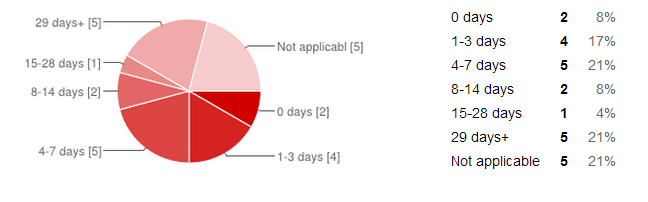
\includegraphics[width=120mm]{Figures/LurkingResponse.png}
\caption{Lurking Response}
\label{overflow}
\end{figure}



\subsubsection{Funding Models}
Within a sample size of 24, a high degree of variance in the types of funding models of open source projects has been observed from analysis of the survey results. 22\% of the responses indicate that funding was received from a for-profit source such as through venture capital investment (7\%) or a direct funding from a for-profit corporation (15\%). On the contrary, a large subset of the surveyed indicated that their funding came from non-profit sources. 24\% of the respondents indicated their project was backed by academic or research grants, 22\% responded that the funding came from donation sources and 17\% responded that the project was financially backed by the members of the core team. The remaining 15\% of the responses indicated that the projects were funded through a crowdfunding campaign such as Kickstarter or Indiegogo.


\subsubsection{Licenses}

73\% of respondents (16 out of 22) reported that they do not know or care about the type of license used in the project. Out of the 27\% (6 out of 22) respondents who reported that they care, one respondent only contributes to copyleft-licensed projects and five respondents only contribute to free software projects (permissive or copyleft). The four largest contributors by number of commits (out of the 22) only contribute to free software.
